\chapter{Benutzeranleitung}
\section{Einleitung}
Wazuh kann zwar Alerts für jegliche Logdateien generieren und anzeigen lassen, die Erkennung eines Incident muss jedoch weiterhin von Fachpersonen gemacht werden.
Dies ist leichter gesagt als getan.
Bei jedem \acrshort{siem} System gibt es auch sogenannte ``False Positives'', Alerts die angezeigt werden aber eigentlich keine Incidents sind und ``False Negatives'', Incidents die keine Alerts generieren.
Die ``False Negatives'' entdecken ist schwierig und kann nur durch verbessern der Wazuh Rules erreicht werden.
Bei den ``False Positives'' kann man durch Untersuchung der betroffenen Entitäten feststellen, ob es sich wirklich um einen Incident handelt.\\

In diesem Kapitel wird angeschaut, wie man im Wazuh Web \acrshort{gui} mit Queries die Alerts filtern kann, es werden Beispiele von realen Attacken aufgezeigt und wie man ``False Positives'' erkennen kann.

\section{Queries}
Das Filtern der Alerts wird in Wazuh mittels der \acrfull{kql} gemacht.
Der Wazuh Manager unterstützt das schreiben dieser Queries mit einem kleinen Interface, wo man die Filter zusammenklicken kann.\\

Dieses Interface befindet sich bei den Security Events im Reiter ``Dashboard'' und ``Events''.
Events gibt eine bessere Übersicht über alle möglichen Filter und eine bessere auflistung aller Informationen eines Alerts.
\begin{figure}[H]
    \centering
    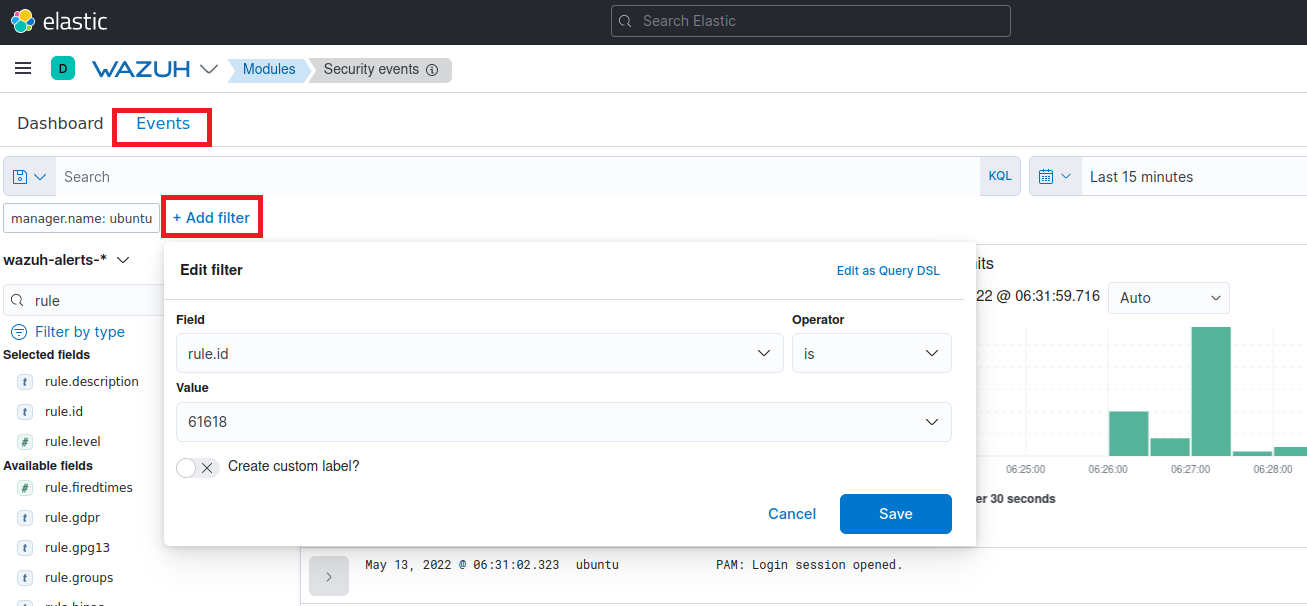
\includegraphics[width=\linewidth]{../img/filter.png}
    \caption{\acrshort{kql} Filter in Wazuh}
\end{figure}

In diesem Interface kann nun das Feld ausgewählt werden, die Art des Vergleichst und der Wert.
Im Bild oben werden zum Beispiel nur noch Rules angezeigt, welche die ID 61618 haben.
Auf diese Weise kann man auch unnötige Rules ausblenden, oder nur bestimmte Rules eines bestimmten PCs anzeigen.

\section{Attacken Beispiele}
Attacken mit und ohne Kompromittierung generieren oftmals einen Level 12 Alert. Daher lohnt es sich, täglich die Level 12 Alerts in Wazuh anzuschauen.
Um nach diesen zu Filtern gibt es unter Security Events im Reiter ``Dashboard'' einen Shortcut:
\begin{figure}[H]
    \centering
    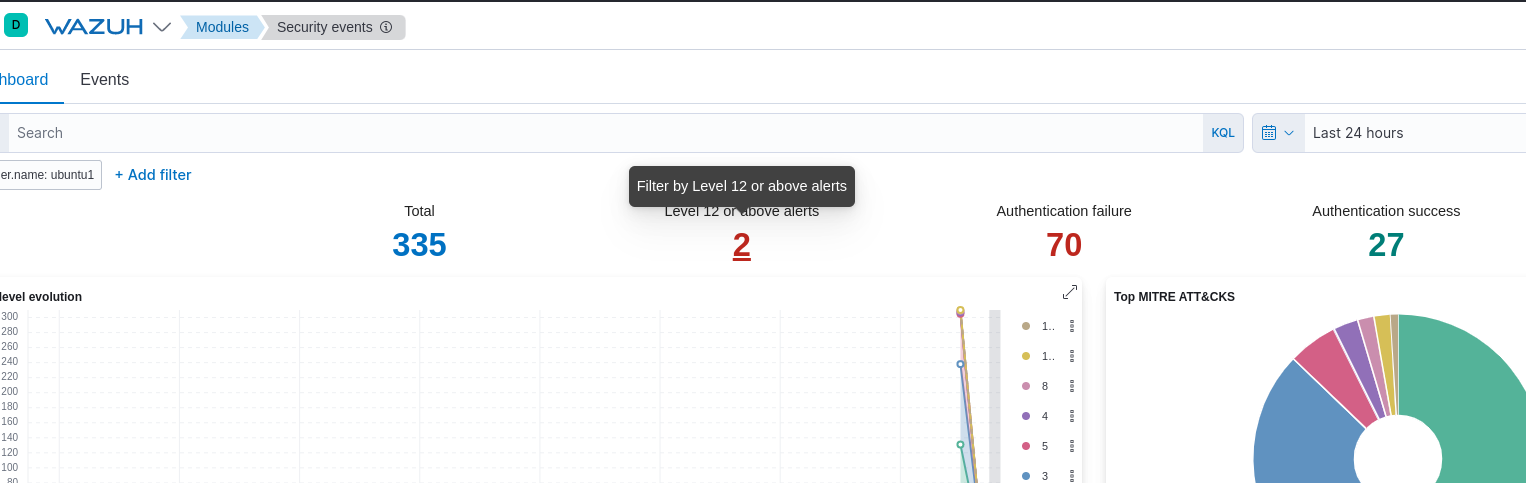
\includegraphics[width=\linewidth]{../img/filter-by-level12.png}
    \caption{Level 12 Alerts Filter}
\end{figure}


\subsection{Mimikatz}
Mimikatz ist eine Software mit welcher es möglich ist, die gespeicherten Passwort Hashes von Benutzern auf Windows auszulesen.
Mit diesem Hash kann dann zum Beispiel eine \href{https://en.wikipedia.org/wiki/Pass\_the\_hash}{Pass-The-Hash}\footnote{Link: https://en.wikipedia.org/wiki/Pass\_the\_hash} Attacken ausgeführt werden.\\

Mimikatz Attacken sind besonders gefährlich wenn Sie unentdeckt bleiben und sich auf dem kompromittierten System zuvor ein Domänen Administrator angemeldet hat.
\begin{figure}[H]
    \centering
    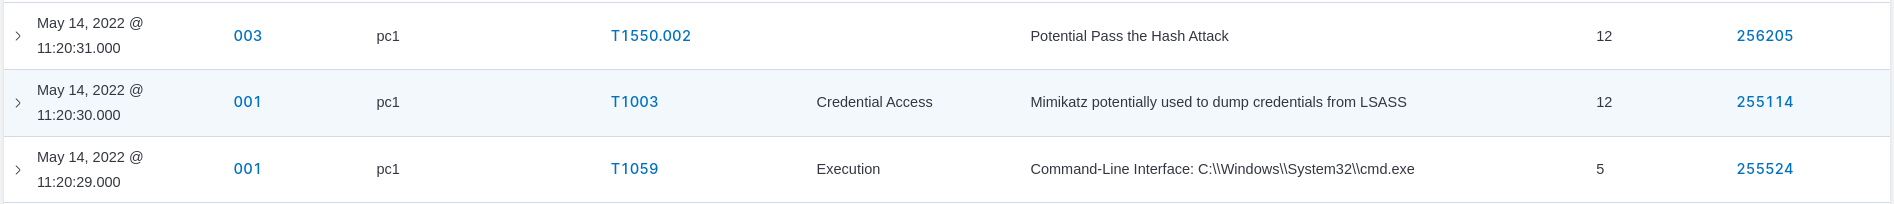
\includegraphics[width=\linewidth]{../img/mimikatz.png}
    \caption{Mimikatz Attacke in Wazuh}
\end{figure}

\subsubsection{Reaktion}
Bei einer Mimikatz Attacke sollten die Domänenadministratoren deaktiviert und die Passwörter dieser zurückgesetzt werden.

\subsubsection{Prävention}
Ein effektiver Weg sich gegen eine Mimikatz Attacke zu schützten, ist \acrshort{laps} auf den Computern zu installieren. 
Ausserdem sollten möglichst wenige Domänenaccounts Administrator auf mehreren Computer sein.
Genauere Anleitungen dazu befinden sich im Dokument ``Security Best Practices'' in diesem GitHub Repository.

\subsection{Brute Force}
Attacken können auch Alerts mit anderen Leveln auslösen. 
Eine SSH Brute Force Attacke löst zum Beispiel einen ``sshd: authentication failed.'' Alert mit Level 5 aus.
Wenn zu viele von diesen Alerts in kurzer Zeit ausgelöst werden, gibt es einen ``sshd: Multiple authentication failures.'' Alert mit Level 10.\\

Dadurch stand das betroffene System wahrscheinlich unter Angriff, aber noch ohne Erfolg.
Wenn ein Angreifer erfolgreich ist, wird eine ``Multiple authentication failures followed by a success.'' Alert mit Level 12 ausgelöst.
\begin{figure}[H]
    \centering
    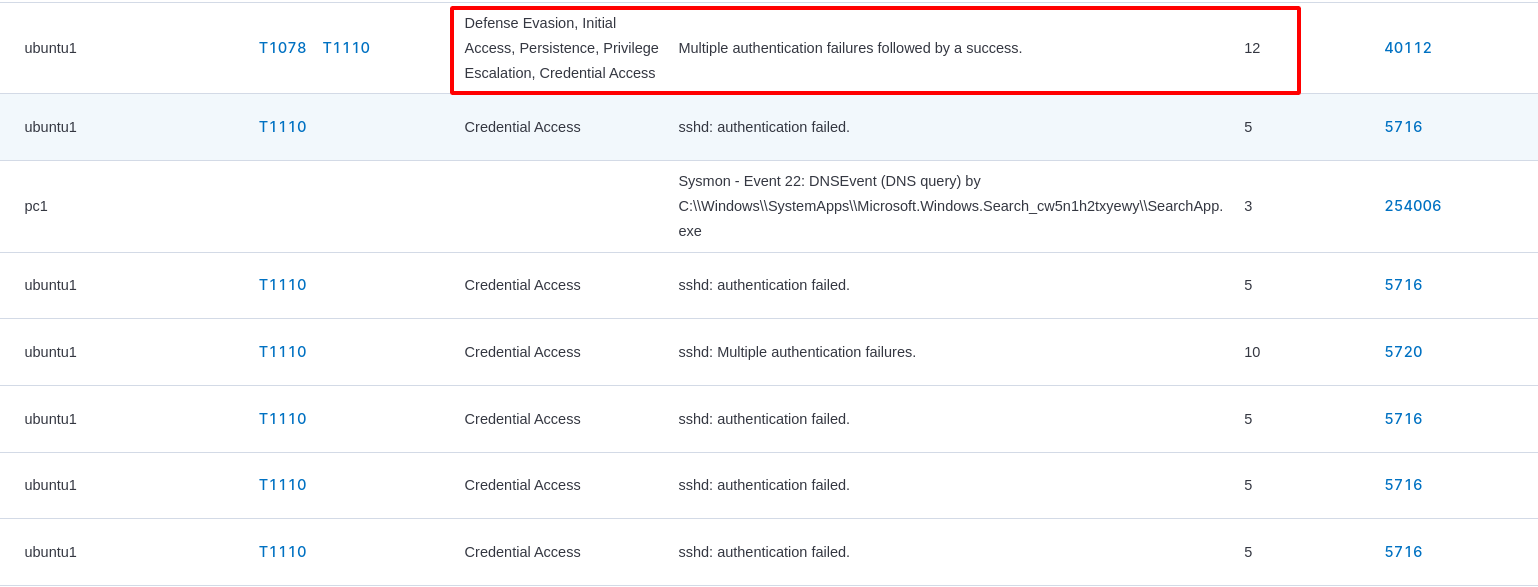
\includegraphics[width=\linewidth]{../img/brute-force.png}
    \caption{Brute Force Attacke in Wazuh}
\end{figure}

\subsubsection{Reaktion}
Bei einer Brute Force Attacke sollten alle Daten gesammelt werden.
\begin{itemize}
    \item Welches Gerät wurde von welcher IP angegriffen?
    \item Ist die Brute Force Attacke per SSH, RDP, physisch beim Windows Login oder über andere Wege? 
    \item Befindet sich der Angreiffer im lokalen Netzwerk oder extern?
\end{itemize}

Dadurch kann man definieren, wie die Brute Force Attacken geblockt werden können.

\subsubsection{Prävention}
Die beste Prävention gegen Brute Force Attacken ist eine gute Passwortrichtlinie und somit starke Passwörter von Benutzern.
Genauere Anleitungen dazu befinden sich im Dokument ``Security Best Practices'' in diesem GitHub Repository.

\section{False Positives}
False Positives können am besten durch genauere Untersuchen der Alerts festgestellt werden.
Eventuell hat ein Benutzer sein Passwort vergessen und erst beim 10. mal richtig eingegeben. 
Daher sollte man mit den Benutzern der Systeme Kontakt aufnehmen, falls die Möglichkeit besteht, dass es ein legitimer Fehler eines Benutzers war.  

\subsection{Check Hash}
Angreiffer benutzen gerne bekannte Namen von Betriebssystem Dateien, um ihre Schadsoftware zu verdecken.
Der Name kann zwar gefälscht werden, jedoch ändert sich der Hash der Datei damit.
Durch überprüfen des Hashs kann festgestellt werden, ob es sich um die legitime Datei handelt. \\

Wazuh logt bei Alerts von ausgeführten Prozessen auch den Hash mit.
In diesem Beispiel wurde der Prozess svchost.exe ausgeführt:
\begin{figure}[H]
    \centering
    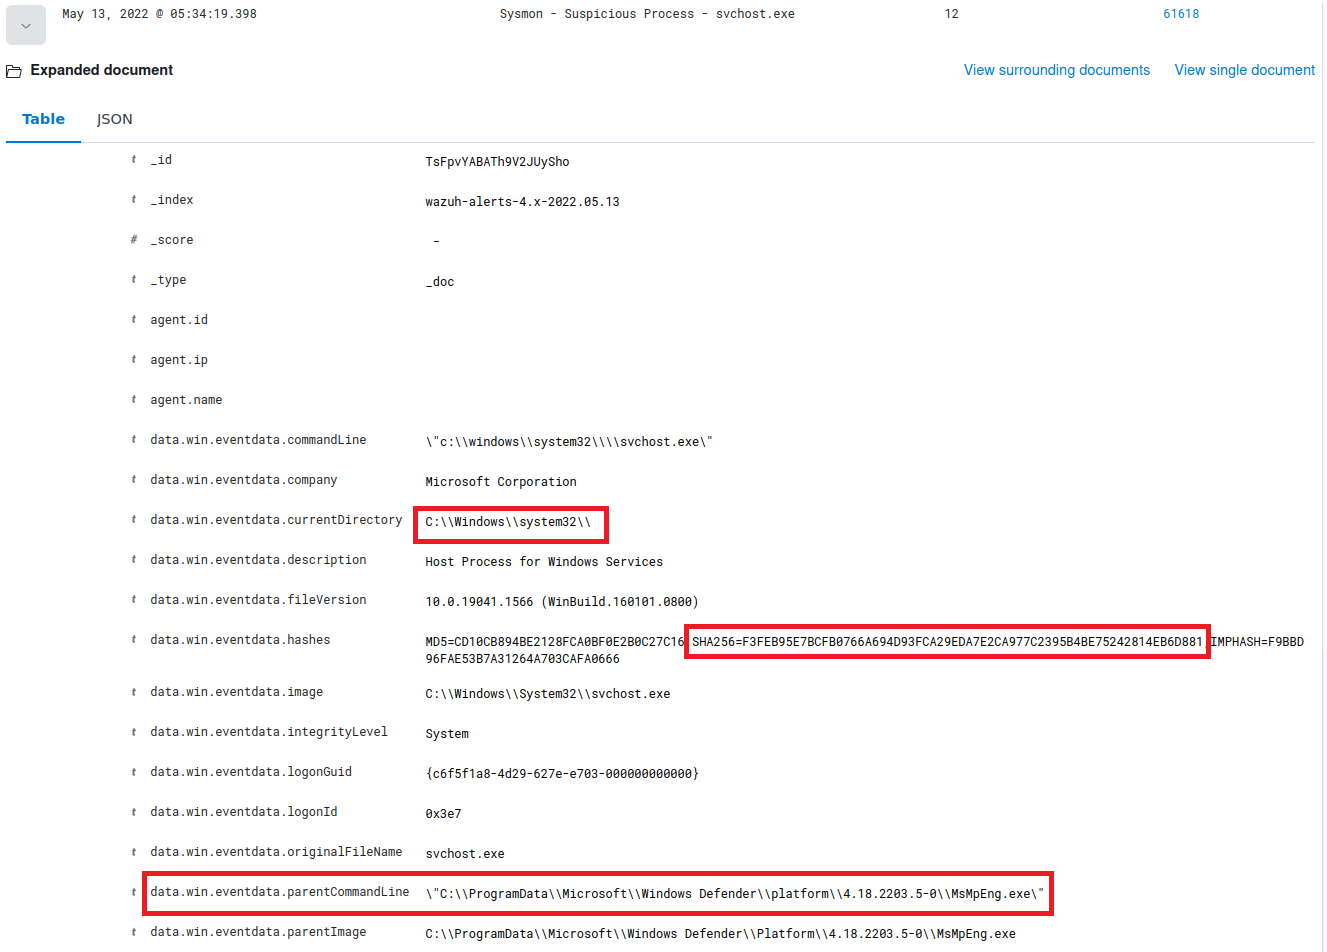
\includegraphics[width=\linewidth]{../img/check-hash-1.png}
    \caption{Hash vergleichen}
\end{figure}

Windows hat ein eingebautes Tool, um den Hash von Dateien zu berechnen.
Dieses heisst ``certutil''.
Damit kann der Hash von einer nicht komprimittierten svchost.exe Datei berechnet und verglichen werden.
Dabei muss jedoch beachtet werden, dass es sich auch um die gleiche Version der .exe Datei handelt.

\begin{lstlisting}
    certutil -hashfile "C:\Windows\System32\svchost.exe" SHA256
    #Hash: f3feb95e7bcfb0766a694d93fca29eda7e2ca977c2395b4be75242814eb6d881
\end{lstlisting}

Alternativ gibt es auch Online Tools wie \href{https://www.virustotal.com/gui/home/upload}{VirusTotal}\footnote{Link: https://www.virustotal.com/gui/home/upload}, bei welchen die Datei, ein URL oder der Hash abgefragt werden können.